% Template for ICASSP-2016 paper; to be used with:
%          spconf.sty  - ICASSP/ICIP LaTeX style file, and
%          IEEEbib.bst - IEEE bibliography style file.
% --------------------------------------------------------------------------
\documentclass{article}
\usepackage{spconf,amsmath,graphicx,bm,setspace}
\usepackage{todonotes}
\setlength{\marginparwidth}{1.5cm}
\usepackage{lipsum}
\usepackage{graphicx}
\graphicspath{{images/}}

% ADD THE FOLLOWING COUPLE LINES INTO YOUR PREAMBLE
\let\OLDthebibliography\thebibliography
\renewcommand\thebibliography[1]{
  \OLDthebibliography{#1}
  \setlength{\parskip}{0pt}
  \setlength{\itemsep}{0pt plus 0.3ex}
}

% Example definitions.
% --------------------
\def\x{{\mathbf x}}
\def\L{{\cal L}}

% Title.
% ------
\title{Knowledge Transfer and Boosting Approach to \\Prediction of Affective Dimensions in Movies}
%
% Single address.
% ---------------
\name{Rahul Gupta, Shrikanth Narayanan, Sabyasachee Baruah}
\address{Signal Analysis and Interpretation Lab,
        University of Southern California,  
  Los Angeles, CA, USA}  
\begin{document}
\ninept
%
\maketitle
%
\begin{abstract}
   Put abstract here 
 
\end{abstract}
%
\begin{keywords}
Gradient Boosting, Knowledge Transfer, Valence, Arousal
\end{keywords}
%
\section{Introduction}
\label{sec:intro}

\section{Background}


\section{Dataset}
The data is taken from the LIRIS-ACCEDE(Annotated Creative Commons Emotional DatabaseE for affective video content analysis) database \cite{baveye2015liris} presented in the 2016 MediaEval Emotional Impact of Movies Task. The dataset contains 30 short films of length varying from 3 to 28 minutes, each with a valence and arousal label in the range -1 to 1 for every second, annotated by 10 participants.

\indent  A variety of visual, speech and music features are used for training our model. The visual features used are luminance, intensity and optical flow. The speech features are mel-frequency cepstral coefficients, voice probability, zero crossing rate, harmonic to noise ratio, fundamental frequency and energy logarithm. We also include the first and second derivative, and the arithmic mean and standard deviation of the countour of the signal for every speech feature. Lastly we compute 12 semitones for our musical chroma features. We have used the OpenSMILE toolbox for feature extraction. A total of 9 statistics - mean, median, standard deviation, kurtosis, lower and upper quartile, minimum, maximum and range are computed for every feature. We choose a 10 second wide sliding window for calculating our statistics. In total we have 156 visual, speech and musical features, each with nine statistics, thus ending up with a dimension of 1404 for our feature matrix.

\section{Methodology}


\subsection{Baseline}
The features and annotations are available at different time frequencies. The video and audio features have been extracted at a rate of 30 and 100 values per second respectively, whereas the ground truth is annotated for each second. To align both these sequences together, we calculate the aforementioned nine statistics over a sliding window on the feature array and assign the computed feature vector of dimension 1404 to the time second at the center of the window. Concordance correlation coefficient is employed as the evaluation metric. We observe the variation in performance for different models on baseline performance as shown in tables \ref{Valence_table} and \ref{Arousal_table}. 

\indent Farther analysis of the performance of the baseline models shows the variation in performance across the movies, as shown in figure \ref{comparison}. The movies in our dataset span a wide variety of genres (figure \ref{genre}) and enough training data is not available for each type of movie. One of the examples is the film, \textit{To Claire From Sonny}, which is the only romantic movie in the dataset and thus doesn't match any of the movies in the training set in genre, leading to inaccurate predictions of valence and arousal (shown in the figure \ref{comparison}). To overcome this problem we require a much larger dataset that should have enough variation to be representative of the different genres of the LIRIS-ACCEDE dataset, but should also be compatible so that the knowledge gathered (trained model) can be used to predict the affective labels in the original dataset.

\indent To this affect we make use of the Discrete LIRIS-ACCEDE dataset. It contains 9800 short video clips of length 8-12 seconds. The clips have been taken from 160 movies. The ground truth consists of a single global valence and arousal label, unlike the previous dataset, in the range 1 to 5, annotated by 1517 annotators from 89 different countries using crowdsourcing. The differences are shown in table \ref{differences}.

\begin{table}[h]
\centering
\begin{tabular}{|l|p{2.2cm}|p{2.2cm}|}
\hline
				& Continuous LIRIS-ACCEDE	& Discrete LIRIS-ACCEDE \\ \hline
Duration			& 3 - 28 minutes			& 8 - 12 seconds		\\ \hline	
Global/Continuous	& Continuous				& Global 				\\ \hline
Range			& -1 to 1					& 1 to 5				\\ \hline
\end{tabular}
\caption{Differences between Continuous LIRIS-ACCEDE and Discrete LIRIS-ACCEDE.}
\label{differences}
\end{table}

\subsection{Proposed method}

\subsubsection{Knowlege transfer}
We extract the same set of features for the short video clips of Discrete LIRIS-ACCEDE as we had done for the movies of Continuous LIRIS-ACCEDE. We train a model on the 9800 videos and predict single values of valence and arousal for each second for the movies. To scale the predictions from the range $[1,5]$ to $[-1,1]$, we use linear modeling by minimizing the squared error between the true labels and predictions. 

\subsubsection{Gradient boosting}
We have used the knowledge gathered from the videos of Discrete LIRIS-ACCEDE to predict the labels of a different dataset, Continuous LIRIS-ACCEDE. However the huge difference in duration between the video clips and movies means that the model cannot still account for the effect of past scenes on the emotions felt by the viewer at the moment. Knowledge transfer predicts the sequence of labels based only on the feature vector of the corresponding second. We leverage the features of the movies to take care of the effect of history while experiencing emotions in viewing a movie.

We calculate the pseudo-residual error, the difference of the predictions of knowledge transfer and the ground truth. This difference sequence becomes our new target and we train a model on the feature matrix of the movies to predict it. To account for the effect of history on the current annotation of valence and arousal, we shift our feature matrix forward in time relative to the target vector. The delay is found out by maximising mutual information between the shifted feature matrix and target vector. We additionally apply a smooting average filter on our predictions to subtract any noise present in the movie features. We add our predictions of the pseudo-residual error to the output of knowledge transfer to get our new predictions. This process is repeated again until we no longer see an improvement in performance.

\section{Results}
The performance of the baseline models, knowledge transfer and gradient boosting are shown in tables \ref{Valence_table} and \ref{Arousal_table}. Figure \ref{comparison} compares the performance of baseline models and gradient boosting technique, in both valence and arousal, across the 30 movies of the LIRIS-ACCEDE dataset. \textit{To Claire From Sonny} is a movie from the dataset and has been labelled in the figure. Figure \ref{genre} shows the distribution of genres in the same dataset.
\begin{table}[h]
\centering
\begin{tabular}{|l|l|l|l|}
\hline
						& RMSE		& Correlation 	& CCC 	 \\ \hline
Linear 					& 0.344		& 0.143		& 0.058  \\ \hline	
Linear (feature selection)		& 0.339		& 0.200 		& 0.075	 \\ \hline
Ridge					& 0.344 		& 0.122		& 0.039	 \\ \hline
Ridge (feature selection)		& 0.344		& 0.121		& 0.044	 \\ \hline
NN						& 0.330		& .363		& 0.116 \\ \hline
& & & \\ \hline
Knowledge transfer 		& 0.331		& 0.295		& \textbf{0.128}	 \\ \hline
Gradient boosting 			& 0.342 		& 0.208 		& \textbf{0.128}  \\ \hline
\end{tabular}
\caption{Results for Valence. The bold numbers shows the improvement.}
\label{Valence_table}
\end{table}

\begin{table}[h]
\centering
\begin{tabular}{|l|l|l|l|}
\hline
						& RMSE		& Correlation 	& CCC 	 \\ \hline
Linear					& 0.286		& 0.171		& 0.064  \\ \hline	
Linear (feature selection)		& 0.278		& 0.305 		& 0.113	 \\ \hline
Ridge					& 0.288  		& 0.141		& 0.030	 \\ \hline
Ridge (feature selection)		& 0.279		& 0.293		& 0.097	 \\ \hline
NN						& 0.296		& 0.092		& 0.023 \\ \hline
& & & \\ \hline
Knowledge transfer 		& 0.299		& 0.249 		& \textbf{0.221}	 \\ \hline
Gradient boosting 			& 0.277 		& 0.334 		& \textbf{0.270}  \\ \hline
\end{tabular}
\caption{Results for Arousal. The bold numbers shows the improvement.}
\label{Arousal_table}
\end{table}

\begin{figure}[h]
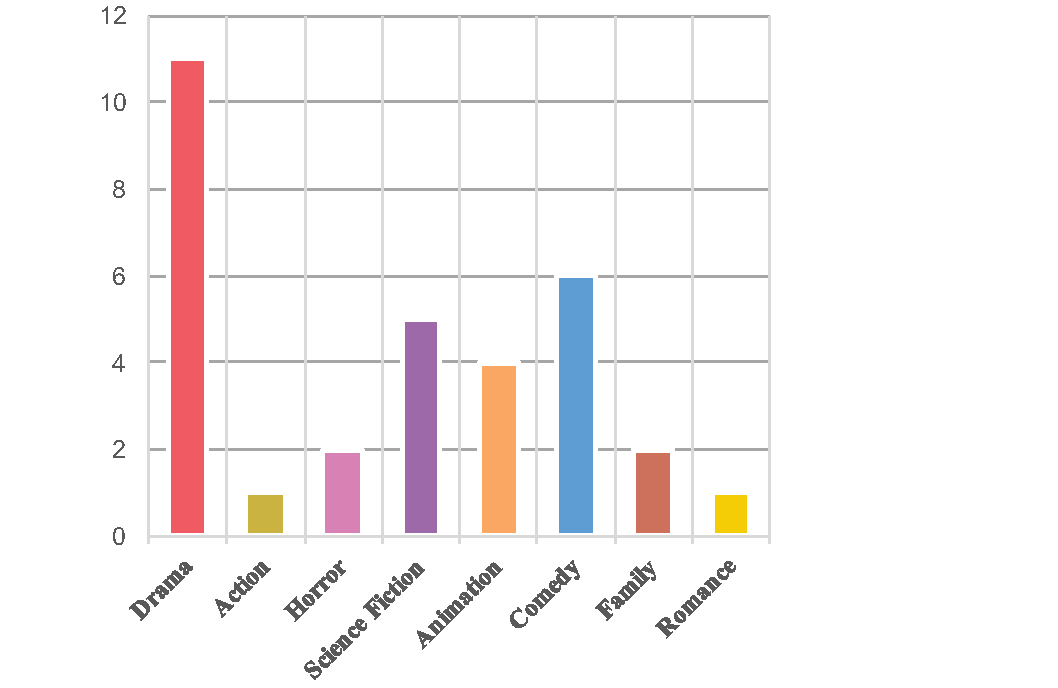
\includegraphics[width=10cm]{genre}
\centering
\caption{Distribution of genre in LIRIS-ACCEDE Dataset}
\label{genre}
\end{figure}

\begin{figure*}[h]
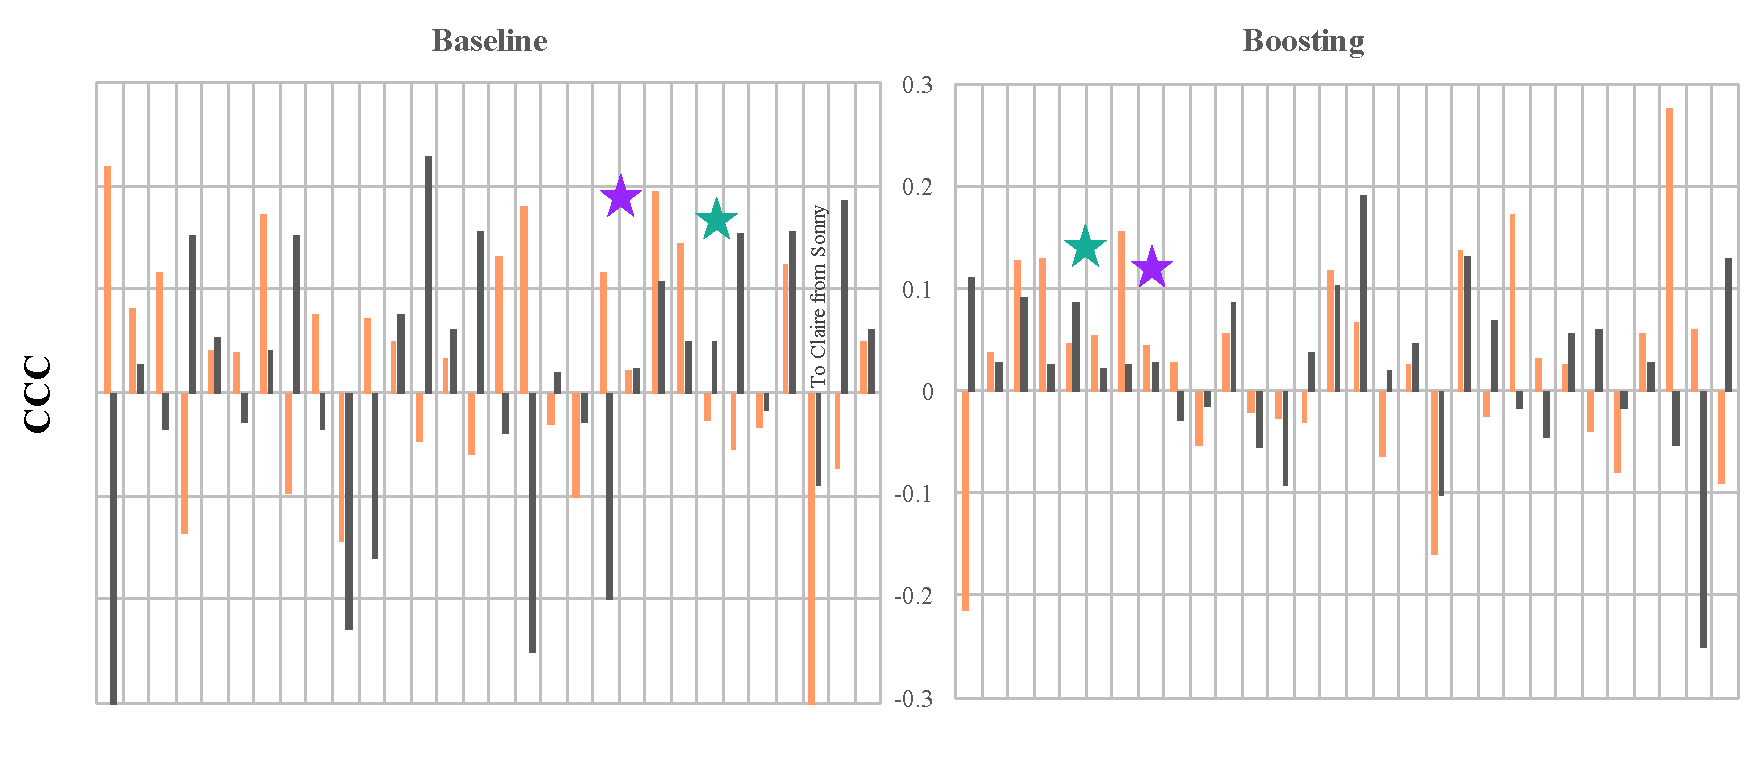
\includegraphics[width=\textwidth, height = 8cm]{comparison}
\centering
\caption{Performance of Baseline models and Gradient Boosting method across the 30 movies}
\label{comparison}
\end{figure*}

\subsection{Discussion}
We can observe the improvement in performance of Knowledge Transfer and Gradient Boosting compared to the baseline models. Among the baseline models, we observe that the linear models perform best for arousal, whereas neural networks show the best performance in valence prediction. There is no significant improvement for Gradient Boosting over Knowledge Transfer for valence prediction. When we analyze the performance farther across the movies, we observe a more consistent performance for both valence and arousal for gradient boosting compared to baseline. The case of the movie \textit{To Claire From Sonny} has already been discussed, and we can see the improvent in CCC after gradient boosting.

\section{Conclusion}
Knowledge Transfer from a larger and more varied dataset not only improves performance, but also results in more consistent CCC values for different movies. We have used root mean squared error as a proxy for the evaluation of pseudo-residual error for now. We endeavour to use CCC instead in the farther work. 

\footnotesize{
\begin{spacing}{.85 }
%\vfill\pagebreak
% BiBTeX files (here: strings, refs, manuals). The IEEEbib.bst bibliography
% style file from IEEE produces unsorted bibliography list.
% -------------------------------------------------------------------------
\bibliographystyle{IEEEbib2}
\bibliography{refs}
\end{spacing}
}
\end{document}
